\documentclass[12pt,a4paper,oneside]{report}
\usepackage[a4paper,margin=1in]{geometry}
\usepackage[T1]{fontenc}
\usepackage{mathptmx}
\usepackage{graphicx,float,booktabs,array,tabularx,setspace,amsmath}
\usepackage{enumitem,listings,xcolor,titlesec,caption}
\usepackage[hidelinks]{hyperref}
\graphicspath{{figures/}}
\onehalfspacing
\setlength{\parskip}{6pt}
\setlist{itemsep=2pt}
\captionsetup{font={bf,small},labelsep=period,figurename=Figure}
\titleformat{\chapter}[block]{\centering\bfseries\fontsize{18}{22}\selectfont}{}{0pt}{}
\titlespacing*{\chapter}{0pt}{0pt}{18pt}
\titleformat{\section}{\bfseries\fontsize{14}{17}\selectfont}{}{0pt}{}
\renewcommand{\thefigure}{\arabic{figure}}
\renewcommand{\thetable}{\arabic{table}}
\lstset{basicstyle=\ttfamily\footnotesize,backgroundcolor=\color{gray!10},frame=single,
  rulecolor=\color{gray!40},keywordstyle=\color{blue!60!black},language=Python,
  showstringspaces=false,xleftmargin=1em}
\begin{document}

\begin{titlepage}
\centering
{\fontsize{16}{20}\selectfont\bfseries A Comparative Study of RNN, LSTM, GRU and BiLSTM Models for Sentiment Analysis of IMDB Movie Reviews\par}
\vspace{1.2cm}
Project submitted to the\\
SRM University -- AP, Andhra Pradesh\\
for the partial fulfillment of the requirements to award the degree of\\[0.6cm]
{\bfseries Bachelor of Technology}\\
In\\
{\bfseries Computer Science and Engineering}\\
{\bfseries School of Engineering and Sciences}\\[1cm]
{\bfseries HARSHA SIVA AKASH SALADI \quad AP23110011490}\\
{\bfseries KISHAN BHIMAVARAPU \quad AP23110011351}\\[1cm]

\includegraphics[width=0.38\textwidth]{srm_logo.png}\\[0.8cm]
Under the Guidance of\\
{\bfseries Dr. Lalit Kumar}\\
Assistant Professor, Department of CSE\\
SRM University--AP\\
Neerukonda, Mangalagiri, Guntur\\
Andhra Pradesh -- 522 240\\[0.8cm]
{\bfseries November, 2026}
\end{titlepage}

\begin{center}{\fontsize{19}{23}\selectfont\bfseries Certificate}\end{center}
\vspace{0.5cm}
\hfill Date: \underline{\hspace{3cm}}
\vspace{1cm}

This is to certify that the work present in this Project entitled ``\textbf{A Comparative Study of RNN, LSTM, GRU and BiLSTM Models for Sentiment Analysis of IMDB Movie Reviews}'' has been carried out by \textbf{Harsha Siva Akash Saladi (AP23110011490) and Kishan Bhimavarapu (AP23110011351)} under my supervision. The work is genuine, original, and suitable for submission to the SRM University -- AP for the award of Bachelor of Technology in \textbf{School of Engineering and Sciences}.

\vspace{3cm}
\noindent\textbf{Supervisor}\\[1cm]
(Signature)\\
Dr. Lalit Kumar\\
Assistant Professor, Department of CSE,\\
SRM University -- AP.
\newpage

\begin{center}{\fontsize{18}{22}\selectfont\bfseries Acknowledgement}\end{center}
\vspace{0.5cm}

The satisfaction that accompanies the successful completion of any task would be incomplete without introducing the people who made it possible and whose constant guidance and encouragement crowns all efforts with success.

We are extremely grateful and express our profound gratitude and indebtedness to our project guide, \textbf{Dr. Lalit Kumar}, Department of Computer Science \& Engineering, SRM University, Andhra Pradesh, for the kind help and for giving us the necessary guidance and valuable suggestions in completing this project work.

\vspace{2cm}
\begin{center}
Harsha Siva Akash Saladi (AP23110011490)\\
Kishan Bhimavarapu (AP23110011351)
\end{center}
\newpage
\tableofcontents
\newpage

\chapter*{Abstract}
\addcontentsline{toc}{chapter}{Abstract}
Sentiment analysis is a Natural Language Processing (NLP) task that automatically classifies the opinion expressed in a piece of text as positive or negative. Because text is sequential data, in which word order changes meaning, recurrent neural networks (RNNs) are a natural choice for this task. However, several recurrent architectures exist, and it is not obvious which one gives the best balance between accuracy and computational cost. This project presents a controlled comparison of four recurrent architectures, namely SimpleRNN, Long Short-Term Memory (LSTM), Gated Recurrent Unit (GRU) and Bidirectional LSTM (BiLSTM), on the IMDB movie review dataset of 50,000 reviews. All models use identical preprocessing (10,000-word vocabulary, sequences of 200 tokens), a 64-dimensional word embedding, 64 recurrent units, dropout and the same training settings, so only the recurrent layer differs. The models are evaluated on 25,000 unseen test reviews using accuracy, precision, recall, F1-score, confusion matrices, training time and parameter count. The gated models clearly outperform the SimpleRNN (83.12\%): LSTM achieves the highest test accuracy of 86.76\%, BiLSTM the highest F1-score of 0.867, and GRU reaches 85.54\% with fewer parameters and less training time. BiLSTM needs about 1.8 times the training time of LSTM without an accuracy gain. The results confirm that gating mechanisms reduce the vanishing gradient problem, and that LSTM or GRU offer the best trade-off for practical sentiment classification.

\noindent\textbf{Keywords:} \textit{Sentiment Analysis, Recurrent Neural Network, LSTM, GRU, Bidirectional LSTM, IMDB, Deep Learning, NLP.}

\chapter*{1. Introduction}
\addcontentsline{toc}{chapter}{1. Introduction}
\section*{1.1 Background}
\addcontentsline{toc}{section}{1.1 Background}
Every day, users publish millions of product reviews, movie reviews, tweets and comments. This text contains valuable information about public opinion, but reading it manually is impossible. Sentiment analysis, also called opinion mining, is the NLP task of automatically deciding whether a text expresses a positive or a negative opinion. It is used by e-commerce platforms such as Amazon and Flipkart to summarise product reviews, by companies to monitor their brand on social media, by customer-support teams to prioritise complaints, and by movie platforms such as IMDB to measure audience reaction.

The main difficulty is that the meaning of a sentence depends on the order and context of its words. For example, ``not good'' has the opposite meaning of ``good'', and in ``the plot was predictable but the music was great'' the clause after ``but'' decides the overall sentiment. Traditional bag-of-words models and feed-forward neural networks ignore this order.

\section*{1.2 Significance and Context}
\addcontentsline{toc}{section}{1.2 Significance and Context}
Recurrent Neural Networks (RNNs) process text one word at a time and keep a hidden state that acts as a memory of the words seen so far, which makes them suitable for sequential data. However, the basic RNN suffers from the vanishing gradient problem, so it forgets information from the beginning of long sequences. Long Short-Term Memory (LSTM) and Gated Recurrent Unit (GRU) networks add gates that control the flow of information, and bidirectional networks read the sequence in both directions. These architectures are core topics of the Deep Learning course (Recurrent Neural Networks, Unfolded RNNs, Seq2Seq, LSTM, GRU and Encoder-Decoder architectures), and this project studies them experimentally on a real-world task.

\section*{1.3 Problem Statement}
\addcontentsline{toc}{section}{1.3 Problem Statement}
Given a movie review written in English, classify it as positive or negative, and determine which recurrent architecture (SimpleRNN, LSTM, GRU or BiLSTM) gives the best trade-off between classification performance, model size and training time.

\section*{1.4 Objectives}
\addcontentsline{toc}{section}{1.4 Objectives}
\begin{itemize}
\item To preprocess the IMDB movie review dataset into fixed-length integer sequences.
\item To implement SimpleRNN, LSTM, GRU and BiLSTM classifiers with an identical overall architecture.
\item To train all models under the same conditions and evaluate them on unseen test data.
\item To compare the models using accuracy, precision, recall, F1-score, confusion matrices, training time and number of parameters.
\item To test the trained models on new, user-written reviews and analyse their behaviour on difficult cases such as negation.
\end{itemize}
\section*{1.5 Scope and Purpose}
\addcontentsline{toc}{section}{1.5 Scope and Purpose}
The project is limited to binary (positive or negative) sentiment classification of English movie reviews. It focuses on lightweight recurrent models that can be trained on a normal laptop CPU in a few minutes, rather than very large Transformer models. Its purpose is to give a clear, reproducible comparison that explains why gated recurrent units are preferred over the basic RNN in practice.

\section*{1.6 Related Work}
\addcontentsline{toc}{section}{1.6 Related Work}
Maas et al. [1] introduced the IMDB Large Movie Review dataset and learned word vectors for sentiment analysis. Bengio et al. [6] showed that learning long-term dependencies with gradient descent is difficult because of vanishing and exploding gradients. Hochreiter and Schmidhuber [2] proposed the LSTM to solve this problem with a gated memory cell. Cho et al. [3] introduced the GRU in the RNN encoder-decoder framework, and Chung et al. [4] found that GRU and LSTM perform comparably on sequence modelling. Schuster and Paliwal [5] proposed bidirectional RNNs. More recently, Transformer models such as BERT [7] reach higher accuracy but require far more computation and memory.

\chapter*{2. Methodology}
\addcontentsline{toc}{chapter}{2. Methodology}
\section*{2.1 Approach}
\addcontentsline{toc}{section}{2.1 Approach}
The project follows an experimental, comparative approach. A single pipeline is built in which every step (data, preprocessing, embedding, classifier head, optimiser, number of epochs and random seed) is fixed, and only the recurrent layer is changed. Any difference in the results can therefore be attributed to the recurrent architecture itself. Figure 2 shows the complete workflow.

\section*{2.2 Dataset}
\addcontentsline{toc}{section}{2.2 Dataset}
The IMDB Large Movie Review dataset [1] contains 50,000 highly polar movie reviews labelled positive (1) or negative (0). It is balanced, with 25,000 reviews of each class, so accuracy is a reliable metric. The standard split was used: 25,000 reviews for training, of which 20\% (5,000) were held out as a validation set, and 25,000 reviews for testing. The test reviews are never seen during training. The dataset is loaded directly through the Keras datasets API, in which every word is already mapped to an integer index ranked by frequency. Figure 1 shows the distribution of review lengths: most reviews are shorter than 300 words, with a long tail of very long reviews.

\begin{figure}[H]\centering
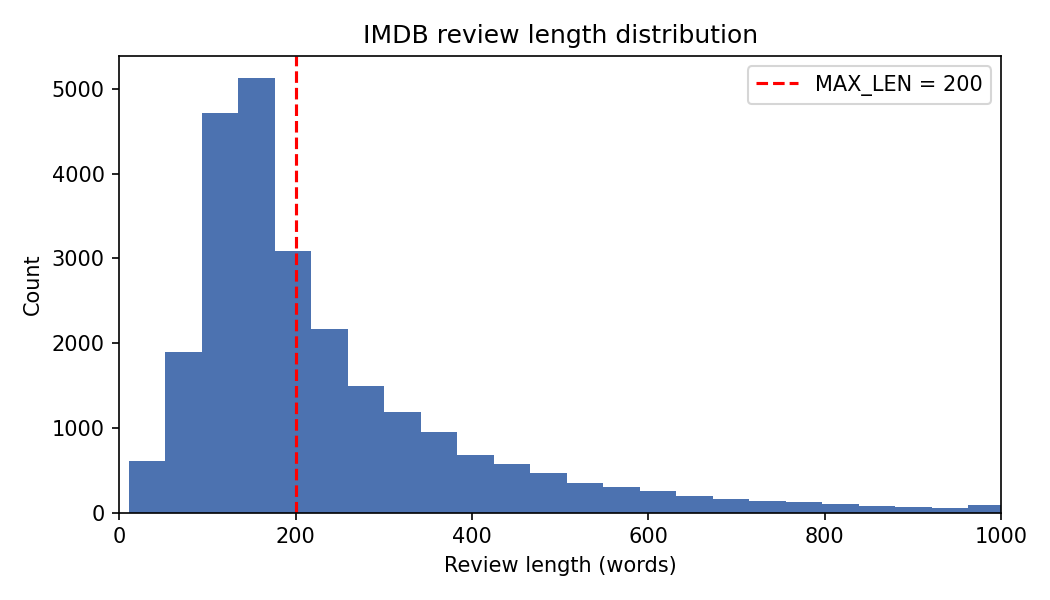
\includegraphics[width=0.88\textwidth]{fig0_review_lengths.png}
\caption{Distribution of review lengths in the training set (dashed line: chosen sequence length of 200)}
\end{figure}
\section*{2.3 Data Preprocessing}
\addcontentsline{toc}{section}{2.3 Data Preprocessing}
\begin{itemize}
\item \textbf{Vocabulary restriction:} only the 10,000 most frequent words are kept, and rarer words are replaced by an 'unknown' token. This removes noise and keeps the embedding small.
\item \textbf{Integer encoding:} each word is represented by its integer index in the vocabulary.
\item \textbf{Padding and truncation:} neural networks need fixed-size inputs, so every review is padded with zeros or truncated to exactly 200 tokens. Pre-padding is used so that the last words of the review stay closest to the output.
\end{itemize}
\section*{2.4 Model Architectures}
\addcontentsline{toc}{section}{2.4 Model Architectures}
All four models share the structure: Input (200 tokens) $\rightarrow$ Embedding (10,000 $\times$ 64) $\rightarrow$ Recurrent layer (64 units) $\rightarrow$ Dropout (0.5) $\rightarrow$ Dense (1 unit, sigmoid). The embedding layer learns a 64-dimensional vector for each word, in which words with similar meaning get similar vectors.

SimpleRNN. At each time step t the hidden state is updated from the current input x\_t and the previous hidden state:

\begin{equation*}h_t = \tanh(W_x x_t + W_h h_{t-1} + b)\end{equation*}
When the network is unfolded over 200 time steps, the gradient is multiplied by W\_h many times during backpropagation through time, so it vanishes and early words receive almost no learning signal.

LSTM. The LSTM adds a separate cell state c\_t that information can flow along almost unchanged, controlled by three gates (forget f\_t, input i\_t and output o\_t), where sigma is the sigmoid function:

\begin{equation*}f_t = \sigma(W_f[h_{t-1},x_t]+b_f),\quad i_t = \sigma(W_i[h_{t-1},x_t]+b_i),\quad o_t = \sigma(W_o[h_{t-1},x_t]+b_o)\end{equation*}
\begin{equation*}c_t = f_t \odot c_{t-1} + i_t \odot \tanh(W_c[h_{t-1},x_t]+b_c),\qquad h_t = o_t \odot \tanh(c_t)\end{equation*}
GRU. The GRU merges the cell state and hidden state and uses only two gates, update z\_t and reset r\_t, so it has fewer parameters than the LSTM:

\begin{equation*}z_t = \sigma(W_z[h_{t-1},x_t]),\quad r_t = \sigma(W_r[h_{t-1},x_t]),\quad h_t = (1-z_t)\odot h_{t-1} + z_t \odot \tanh(W[r_t \odot h_{t-1}, x_t])\end{equation*}
BiLSTM. Two independent LSTMs read the review forwards and backwards, and their final hidden states are concatenated, so every position has context from both sides. The recurrent layer here acts like the encoder of an encoder-decoder (Seq2Seq) model: it compresses the whole review into one fixed-length vector, which is then decoded by the dense layer into a single label (a many-to-one architecture).

Output layer. The final dense layer outputs y = sigmoid(w·h + b), the probability that the review is positive. A threshold of 0.5 gives the predicted class.

\section*{2.5 Experimental Setup}
\addcontentsline{toc}{section}{2.5 Experimental Setup}
\begin{table}[H]\centering\small
\caption{Hyperparameters used for all four models}
\begin{tabularx}{\textwidth}{l>{\raggedright\arraybackslash}X}\toprule
\textbf{Hyperparameter} & \textbf{Value} \\\midrule
Vocabulary size & 10,000 \\
Sequence length & 200 tokens \\
Embedding dimension & 64 \\
Recurrent units & 64 (64 per direction for BiLSTM) \\
Dropout & 0.5 \\
Optimizer & Adam (learning rate 0.001) \\
Loss function & Binary cross-entropy \\
Batch size & 128 \\
Maximum epochs & 5 \\
Early stopping & Validation loss, patience 2, best weights restored \\
Random seed & 42 \\
\bottomrule\end{tabularx}\end{table}
Justification of choices: Adam adapts the learning rate of every parameter and converges quickly without tuning [8]. Binary cross-entropy is the standard loss for a sigmoid output with two classes. Dropout [9] and early stopping are used because recurrent models overfit IMDB within a few epochs. 64 units and 5 epochs keep the training time of each model within a few minutes on a CPU.

\begin{equation*}\mathcal{L} = -\frac{1}{N}\sum_{i=1}^{N}\left[y_i\log\hat{y}_i + (1-y_i)\log(1-\hat{y}_i)\right]\end{equation*}
\section*{2.6 Evaluation Metrics}
\addcontentsline{toc}{section}{2.6 Evaluation Metrics}
\begin{itemize}
\item \textbf{Accuracy = (TP + TN) / (TP + TN + FP + FN):} the fraction of reviews classified correctly.
\item \textbf{Precision = TP / (TP + FP):} of the reviews predicted positive, how many really are positive.
\item \textbf{Recall = TP / (TP + FN):} of the truly positive reviews, how many were found.
\item F1-score = 2 $\times$ Precision $\times$ Recall / (Precision + Recall): the harmonic mean of precision and recall.
\item Confusion matrix, training time (seconds) and number of trainable parameters.
\end{itemize}
\section*{2.7 Software Requirements Specifications}
\addcontentsline{toc}{section}{2.7 Software Requirements Specifications}
\begin{table}[H]\centering\small
\caption{Software and hardware requirements}
\begin{tabularx}{\textwidth}{l>{\raggedright\arraybackslash}X}\toprule
\textbf{Component} & \textbf{Specification} \\\midrule
Operating system & Windows 11 (64-bit) \\
Programming language & Python 3.11 \\
Deep learning framework & TensorFlow 2 / Keras \\
Data handling & NumPy, Pandas \\
Evaluation & scikit-learn \\
Visualisation & Matplotlib, Seaborn \\
Hardware & Standard laptop, CPU only (no GPU required), 8 GB RAM or more \\
Dataset & IMDB Large Movie Review dataset (via keras.datasets) \\
\bottomrule\end{tabularx}\end{table}
\chapter*{3. Implementation}
\addcontentsline{toc}{chapter}{3. Implementation}
\section*{3.1 Implementation Steps}
\addcontentsline{toc}{section}{3.1 Implementation Steps}
\begin{itemize}
\item \textbf{Step 1 --} Environment setup: installed Python 3.11 with TensorFlow, scikit-learn, Pandas, Matplotlib and Seaborn, and fixed all random seeds to 42 for reproducibility.
\item \textbf{Step 2 --} Data loading: loaded the IMDB dataset with a 10,000-word vocabulary using keras.datasets.imdb.
\item \textbf{Step 3 --} Preprocessing: padded or truncated every review to 200 tokens with pad\_sequences.
\item \textbf{Step 4 --} Model construction: wrote a single build(kind) function that returns a SimpleRNN, LSTM, GRU or BiLSTM model with the same embedding, dropout and output layers.
\item \textbf{Step 5 --} Training: trained each model with Adam, binary cross-entropy, batch size 128, a 20\% validation split and early stopping, recording the training time.
\item \textbf{Step 6 --} Evaluation: predicted the 25,000 test reviews and computed accuracy, precision, recall, F1-score and the confusion matrix.
\item \textbf{Step 7 --} Visualisation: generated the training curves, metric comparison chart, confusion matrices and time/parameter charts.
\item \textbf{Step 8 --} Prediction on new reviews: encoded user-written sentences with the IMDB word index and classified them with all four models.
\end{itemize}
\section*{3.2 Design (DFD Diagram)}
\addcontentsline{toc}{section}{3.2 Design (DFD Diagram)}
Figure 2 shows the data flow of the system, from the raw dataset to the final comparison.

\begin{figure}[H]\centering
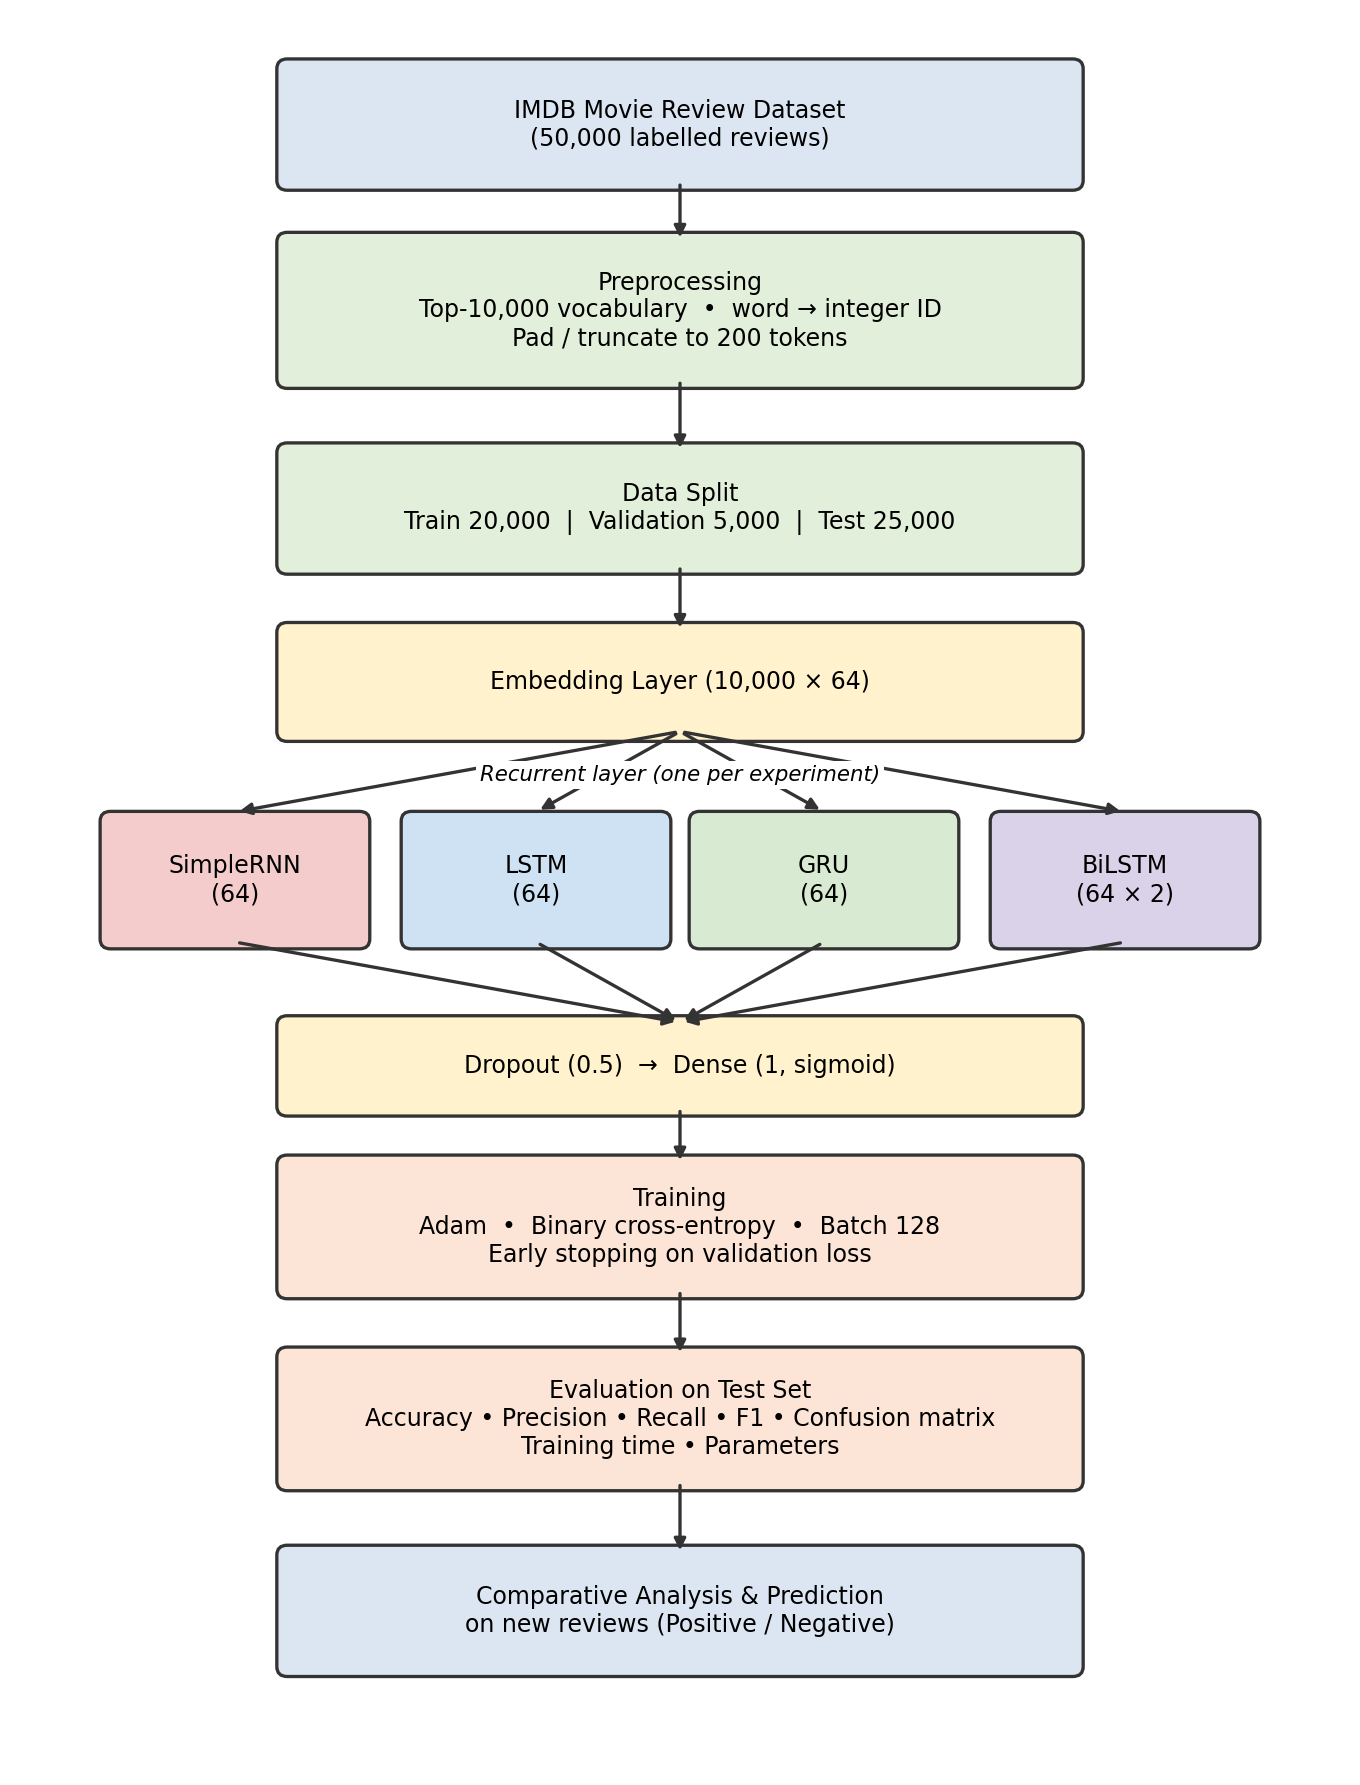
\includegraphics[width=0.73\textwidth]{fig5_system_design_dfd.png}
\caption{System design / data flow diagram of the proposed comparative framework}
\end{figure}
\section*{3.3 Code Snippets}
\addcontentsline{toc}{section}{3.3 Code Snippets}
The core of the implementation is one model-building function, so all four models are guaranteed to be identical except for the recurrent layer:

\begin{lstlisting}
def build(kind):
    m = models.Sequential(name=kind)
    m.add(layers.Input(shape=(MAX_LEN,)))
    m.add(layers.Embedding(VOCAB_SIZE, EMBED_DIM))
    if kind == "SimpleRNN": m.add(layers.SimpleRNN(UNITS))
    elif kind == "LSTM":    m.add(layers.LSTM(UNITS))
    elif kind == "GRU":     m.add(layers.GRU(UNITS))
    elif kind == "BiLSTM":  m.add(layers.Bidirectional(layers.LSTM(UNITS)))
    m.add(layers.Dropout(0.5))
    m.add(layers.Dense(1, activation="sigmoid"))
    m.compile(optimizer="adam", loss="binary_crossentropy",
              metrics=["accuracy"])
    return m
\end{lstlisting}
Each model is trained with early stopping and then evaluated on the test set:

\begin{lstlisting}
es = callbacks.EarlyStopping(monitor="val_loss", patience=2,
                             restore_best_weights=True)
h = model.fit(x_train, y_train, epochs=5, batch_size=128,
              validation_split=0.2, callbacks=[es])
pred = (model.predict(x_test) >= 0.5).astype(int)
print(accuracy_score(y_test, pred), f1_score(y_test, pred))
\end{lstlisting}
\section*{3.4 Challenges and Solutions}
\addcontentsline{toc}{section}{3.4 Challenges and Solutions}
\begin{itemize}
\item \textbf{Variable review length:} reviews range from about 10 to more than 2,000 words. Solved by padding or truncating to 200 tokens, which covers the majority of reviews (Figure 1).
\item \textbf{Overfitting:} training accuracy rose to about 93\% while validation loss started increasing after epoch 2. Solved with dropout (0.5) and early stopping that restores the best weights.
\item \textbf{Long training time on CPU:} BiLSTM takes around 130 seconds per epoch. Solved by using 64 units, a batch size of 128 and at most 5 epochs.
\item \textbf{Fair comparison:} different random initialisations could change the ranking. Solved by fixing the random seed and using the same build function and settings for every model.
\item \textbf{Encoding new sentences:} the IMDB dataset uses an index offset of 3 for special tokens. Solved by shifting the Keras word index by 3 and mapping out-of-vocabulary words to the 'unknown' token.
\end{itemize}
\chapter*{4. Result and Analysis}
\addcontentsline{toc}{chapter}{4. Result and Analysis}
\section*{4.1 Overall Performance}
\addcontentsline{toc}{section}{4.1 Overall Performance}
Table 3 shows the performance of the four models on the 25,000 unseen test reviews, and Figure 3 compares the metrics visually.

\begin{table}[H]\centering\small
\caption{Performance of the four models on the IMDB test set (25,000 reviews)}
\begin{tabular}{lcccccc}\toprule
\textbf{Model} & \textbf{Parameters} & \textbf{Accuracy} & \textbf{Precision} & \textbf{Recall} & \textbf{F1-score} & \textbf{Train time (s)} \\\midrule
SimpleRNN & 648,321 & 0.8312 & 0.8291 & 0.8344 & 0.8317 & 94.8 \\
LSTM & 673,089 & 0.8676 & 0.8791 & 0.8526 & 0.8656 & 295.7 \\
GRU & 665,025 & 0.8554 & 0.8567 & 0.8535 & 0.8551 & 272.0 \\
BiLSTM & 706,177 & 0.8662 & 0.8596 & 0.8755 & 0.8675 & 536.9 \\
\bottomrule\end{tabular}\end{table}
\begin{figure}[H]\centering
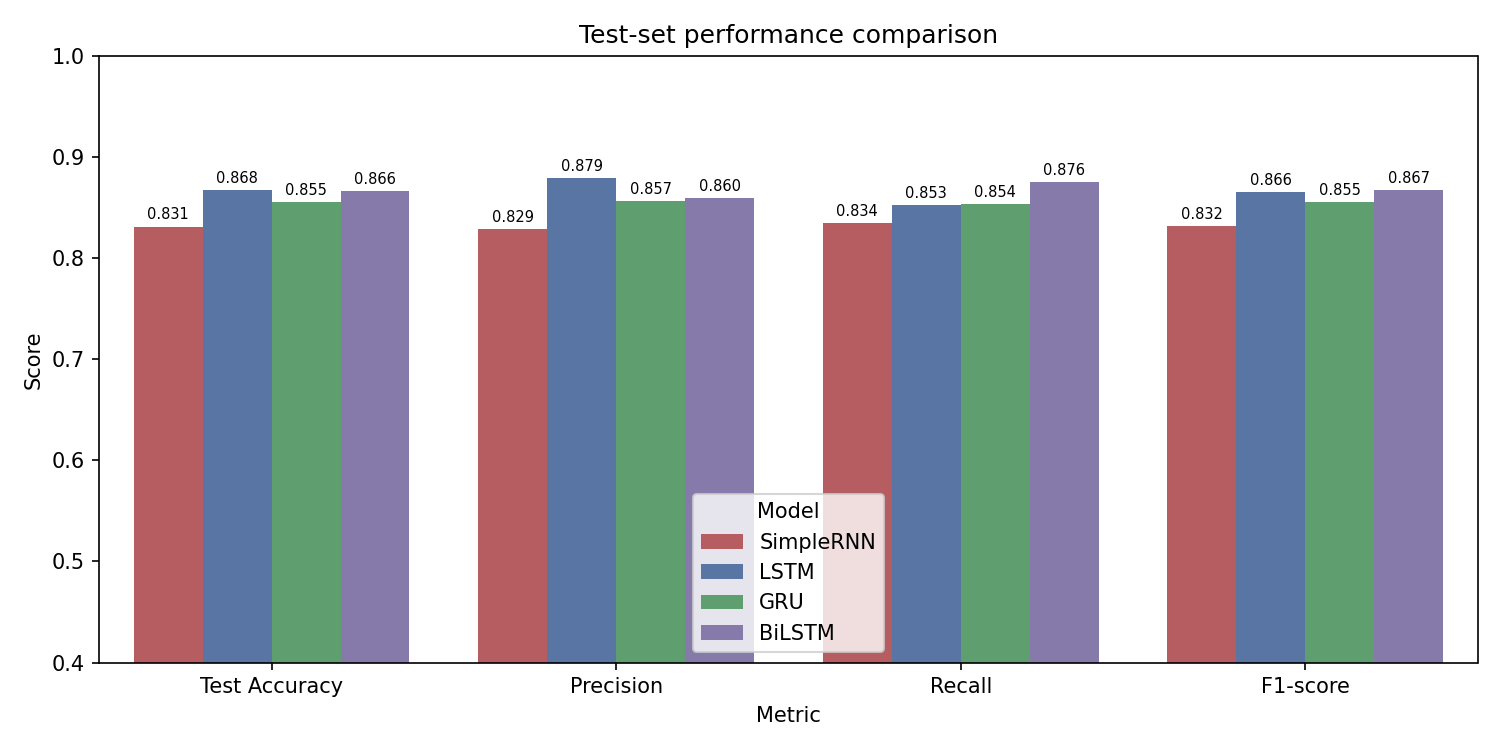
\includegraphics[width=0.96\textwidth]{fig2_metric_comparison.png}
\caption{Test-set accuracy, precision, recall and F1-score of each model}
\end{figure}
LSTM achieves the best accuracy (86.76\%) and precision (0.879). BiLSTM achieves the best recall (0.876) and F1-score (0.867). GRU follows closely with 85.54\%, and SimpleRNN is clearly the weakest at 83.12\%.

\section*{4.2 Training Behaviour}
\addcontentsline{toc}{section}{4.2 Training Behaviour}
\begin{figure}[H]\centering
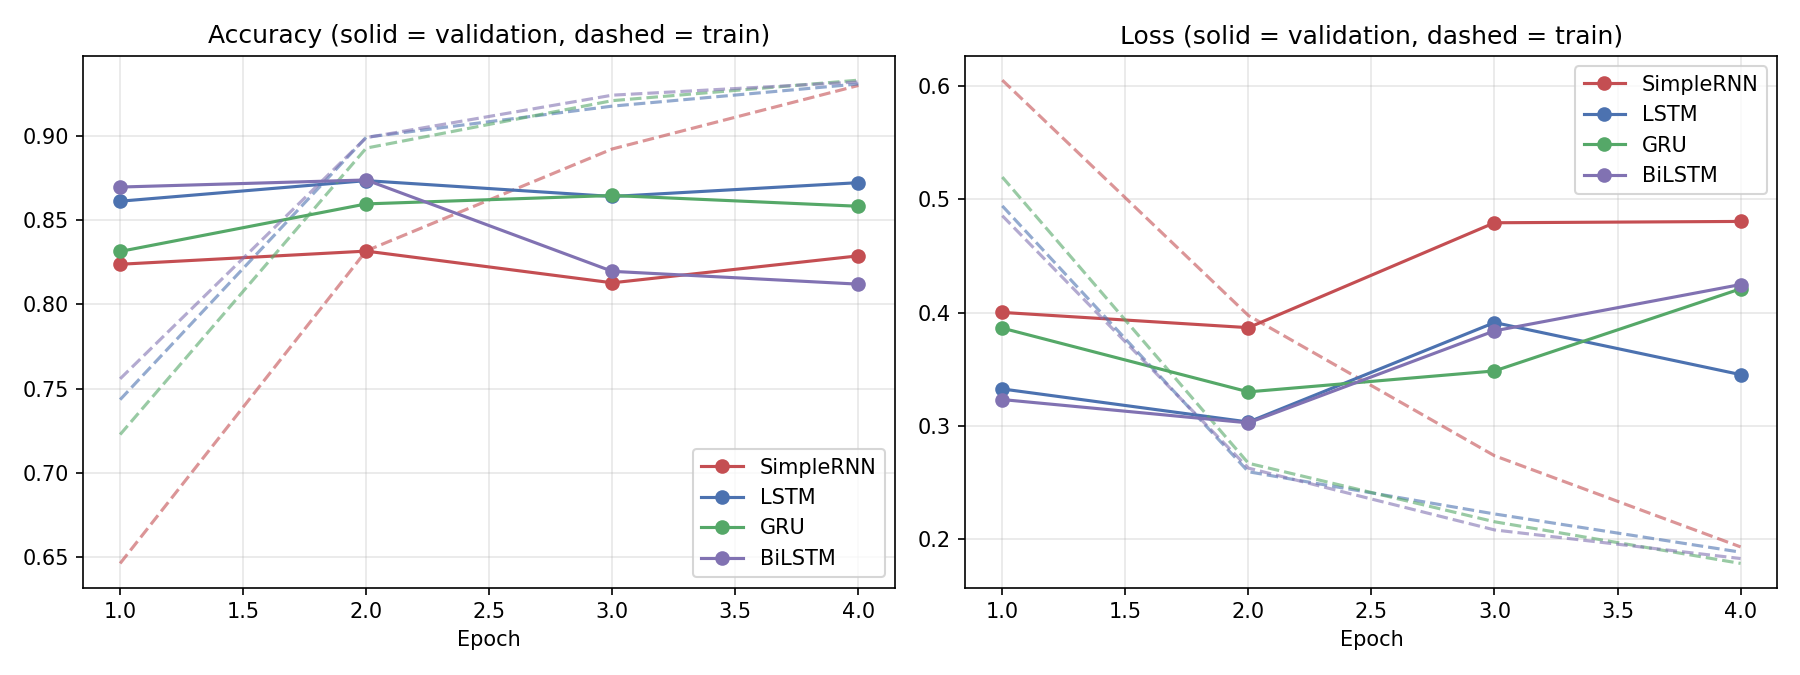
\includegraphics[width=0.96\textwidth]{fig1_training_curves.png}
\caption{Training (dashed) and validation (solid) accuracy and loss per epoch}
\end{figure}
Figure 4 shows that all models reach their lowest validation loss at epoch 2. After that, training accuracy keeps rising towards 93\% while validation loss increases, which is the typical sign of overfitting. Early stopping detected this and restored the epoch-2 weights for every model. SimpleRNN learns slowest (65\% training accuracy after epoch 1) and has the highest validation loss throughout, which reflects its difficulty in using long-range context.

\section*{4.3 Confusion Matrices}
\addcontentsline{toc}{section}{4.3 Confusion Matrices}
\begin{figure}[H]\centering
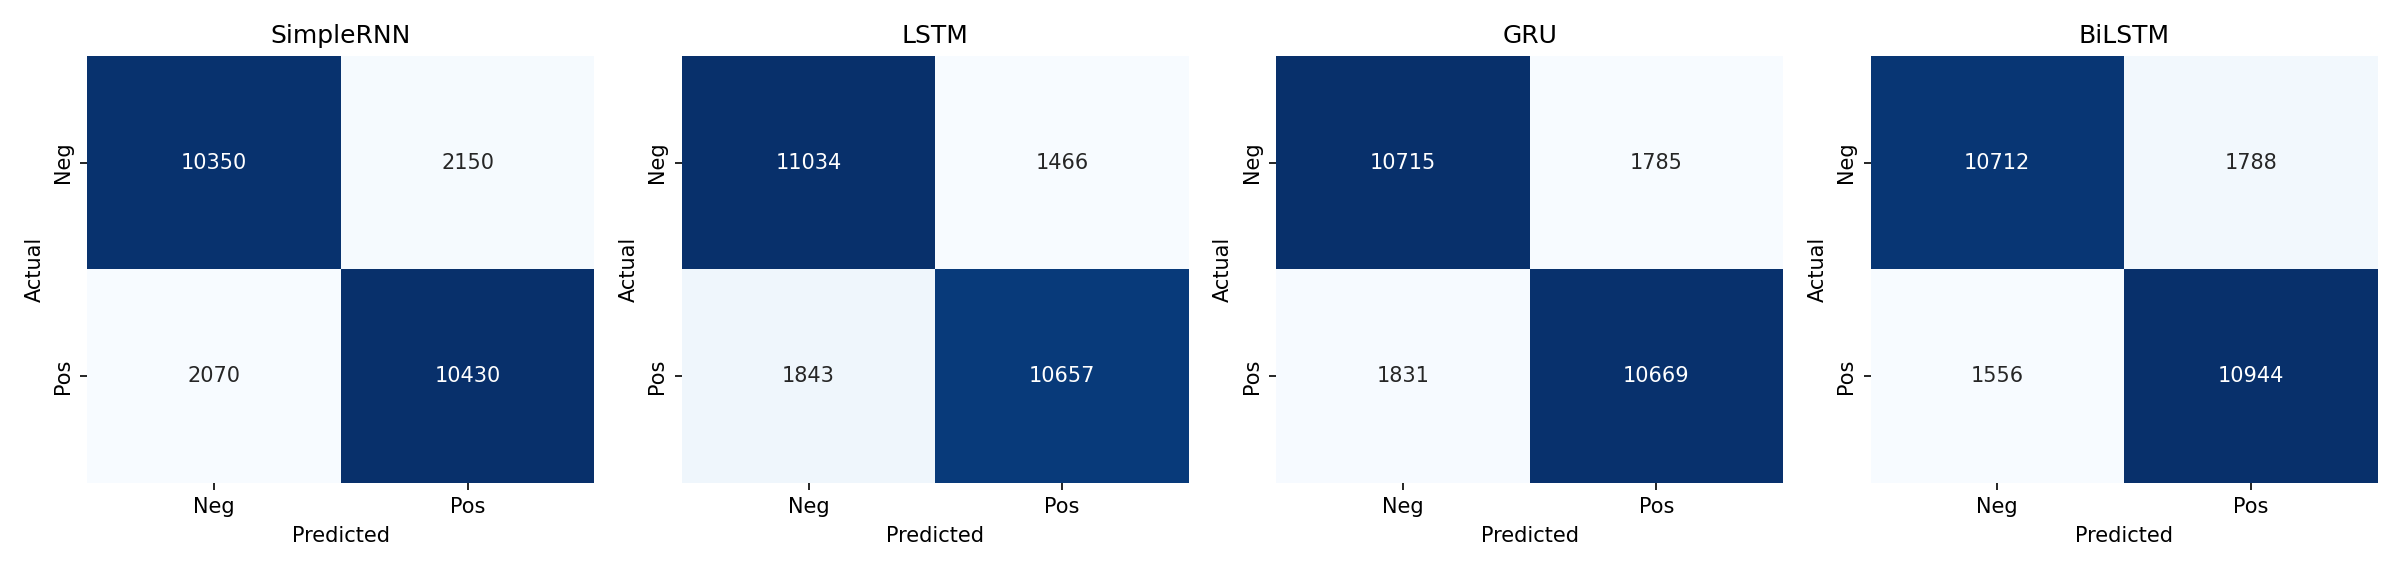
\includegraphics[width=0.96\textwidth]{fig3_confusion_matrices.png}
\caption{Confusion matrices of the four models on the test set}
\end{figure}
The confusion matrices (Figure 5) show that the errors are fairly balanced between the two classes, so none of the models is biased towards one class. LSTM makes the fewest false positives (1,466), while BiLSTM makes the fewest false negatives (1,556), which explains its higher recall.

\section*{4.4 Computational Cost}
\addcontentsline{toc}{section}{4.4 Computational Cost}
\begin{figure}[H]\centering
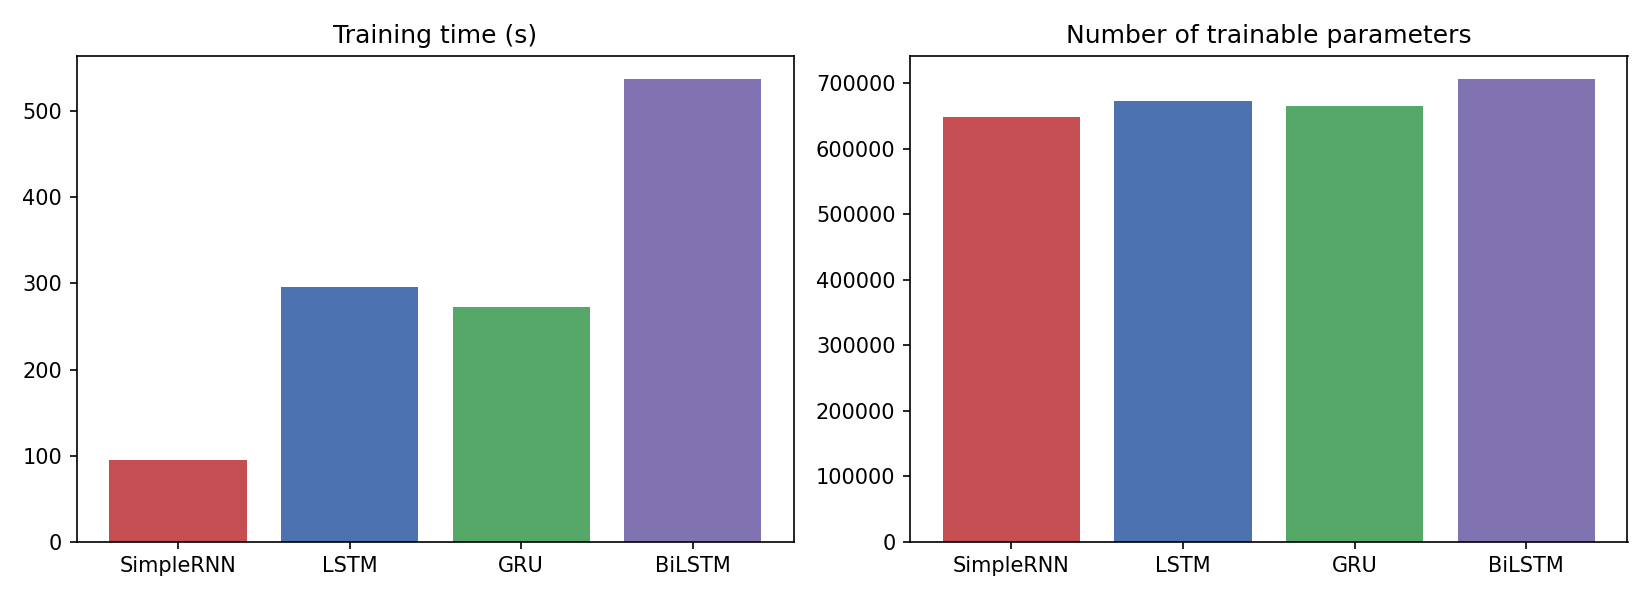
\includegraphics[width=0.96\textwidth]{fig4_time_and_params.png}
\caption{Training time and number of trainable parameters}
\end{figure}
SimpleRNN is the fastest (95 s) because it has a single weight matrix per step. LSTM (296 s) and GRU (272 s) are about 3 times slower, and GRU is about 8\% faster than LSTM. BiLSTM is the most expensive (537 s), about 1.8 times LSTM, because it runs two LSTMs. Most parameters belong to the embedding layer (640,000), so the recurrent layers differ only by 25,000 to 58,000 parameters.

\section*{4.5 Predictions on New Reviews}
\addcontentsline{toc}{section}{4.5 Predictions on New Reviews}
\begin{table}[H]\centering\small
\caption{Predicted label and probability of positive sentiment for new reviews}
\begin{tabularx}{\textwidth}{>{\raggedright\arraybackslash}Xcccc}\toprule
\textbf{Review (written by us)} & \textbf{SimpleRNN} & \textbf{LSTM} & \textbf{GRU} & \textbf{BiLSTM} \\\midrule
This movie was absolutely wonderful, the acting was brilliant and the story was touching & POS (0.62) & POS (0.94) & POS (0.94) & POS (0.92) \\
Worst film I have ever seen. Boring, badly acted and a complete waste of time & NEG (0.01) & NEG (0.01) & NEG (0.00) & NEG (0.01) \\
The plot was predictable but the music and visuals were great & NEG (0.27) & POS (0.71) & POS (0.67) & POS (0.61) \\
I did not like this movie at all, it was not good & NEG (0.08) & POS (0.51) & NEG (0.45) & NEG (0.36) \\
\bottomrule\end{tabularx}\end{table}
All models classify the clearly positive and clearly negative reviews correctly. On the mixed review (``the plot was predictable but the music and visuals were great''), only the gated models understand that the clause after ``but'' dominates, while SimpleRNN predicts negative. The negated sentence (``it was not good'') is the hardest case: GRU and BiLSTM classify it correctly, but LSTM gives a borderline 0.51. This shows that negation is still a challenge for small recurrent models.

\chapter*{5. Discussion and Conclusion}
\addcontentsline{toc}{chapter}{5. Discussion and Conclusion}
\section*{5.1 Comparison with Objectives}
\addcontentsline{toc}{section}{5.1 Comparison with Objectives}
All objectives were achieved: the IMDB data was preprocessed, four recurrent models were implemented with an identical pipeline, trained under the same conditions, evaluated with six measures and tested on new reviews. The initial hypothesis, that gated architectures outperform the basic RNN on long text, was confirmed.

\section*{5.2 Implications of the Findings}
\addcontentsline{toc}{section}{5.2 Implications of the Findings}
\begin{itemize}
\item \textbf{Gating matters:} LSTM, GRU and BiLSTM beat SimpleRNN by 2.4 to 3.6 percentage points, because their gates prevent the vanishing gradient problem and keep sentiment cues from early in the review.
\item \textbf{GRU is the most efficient choice:} it reaches 85.54\%, only 1.2 points below LSTM, with fewer parameters and less training time, which makes it suitable for mobile or low-resource deployment.
\item \textbf{Bidirectionality is not worth its cost here:} BiLSTM gives the best F1-score but no accuracy gain over LSTM, for 1.8 times the training time. For whole-document classification, the final forward state already summarises the review well.
\item \textbf{Regularisation is essential:} every model starts to overfit after two epochs, so early stopping and dropout are necessary even for small models.
\end{itemize}
\section*{5.3 Limitations and Sources of Error}
\addcontentsline{toc}{section}{5.3 Limitations and Sources of Error}
\begin{itemize}
\item Each model was trained once with a single random seed. Small differences such as LSTM versus BiLSTM (0.14 points) may fall within run-to-run variance.
\item Reviews were truncated to 200 tokens, so information at the start of very long reviews is lost.
\item Embeddings were learned from scratch. Pretrained embeddings could improve all models.
\item Only binary sentiment was studied. Neutral, mixed and sarcastic opinions are not modelled.
\item The models struggle with negation, as shown in the new-review test.
\end{itemize}
\section*{5.4 Conclusion}
\addcontentsline{toc}{section}{5.4 Conclusion}
This project compared SimpleRNN, LSTM, GRU and BiLSTM for sentiment analysis of IMDB movie reviews under identical conditions. LSTM achieved the best accuracy (86.76\%), BiLSTM the best F1-score, and GRU nearly matched them at lower cost, while the basic RNN performed worst. The study shows experimentally why gated recurrent units replaced the basic RNN in practice, and that GRU gives the best accuracy-to-cost ratio. Its contribution is a simple, fully reproducible benchmark and code base that can serve as a baseline for more advanced models.

\chapter*{6. Future Scope}
\addcontentsline{toc}{chapter}{6. Future Scope}
\begin{itemize}
\item \textbf{Pretrained word embeddings:} initialise the embedding layer with GloVe or Word2Vec vectors to improve accuracy and generalisation.
\item \textbf{Attention mechanism:} add attention on top of the LSTM/GRU so the model can focus on the most important words, which also makes predictions explainable.
\item \textbf{Transformer models:} compare with BERT, DistilBERT or RoBERTa to quantify the accuracy-versus-cost gap.
\item \textbf{Stacked and hybrid models:} deeper recurrent stacks and CNN-LSTM hybrids.
\item \textbf{Multi-class and aspect-based sentiment:} predict neutral or star ratings, and opinions about specific aspects such as acting or music.
\item \textbf{Multilingual sentiment:} extend to Indian languages such as Telugu and Hindi, and to code-mixed social media text.
\item \textbf{Statistical robustness:} repeat the experiments over several random seeds and report the mean and standard deviation with significance tests.
\item \textbf{Deployment:} package the GRU model as a web or mobile application for real-time review analysis.
\end{itemize}
\chapter*{References}\addcontentsline{toc}{chapter}{References}
\begin{enumerate}[label={[\arabic*]},leftmargin=2.2em]
\item A. L. Maas, R. E. Daly, P. T. Pham, D. Huang, A. Y. Ng and C. Potts, ``Learning Word Vectors for Sentiment Analysis,'' in Proc. 49th Annual Meeting of the Association for Computational Linguistics (ACL), 2011, pp. 142-150.
\item S. Hochreiter and J. Schmidhuber, ``Long Short-Term Memory,'' Neural Computation, vol. 9, no. 8, pp. 1735-1780, 1997. doi: 10.1162/neco.1997.9.8.1735
\item K. Cho et al., ``Learning Phrase Representations using RNN Encoder-Decoder for Statistical Machine Translation,'' in Proc. EMNLP, 2014, pp. 1724-1734.
\item J. Chung, C. Gulcehre, K. Cho and Y. Bengio, ``Empirical Evaluation of Gated Recurrent Neural Networks on Sequence Modeling,'' arXiv:1412.3555, 2014.
\item M. Schuster and K. K. Paliwal, ``Bidirectional Recurrent Neural Networks,'' IEEE Transactions on Signal Processing, vol. 45, no. 11, pp. 2673-2681, 1997.
\item Y. Bengio, P. Simard and P. Frasconi, ``Learning Long-Term Dependencies with Gradient Descent is Difficult,'' IEEE Transactions on Neural Networks, vol. 5, no. 2, pp. 157-166, 1994.
\item J. Devlin, M.-W. Chang, K. Lee and K. Toutanova, ``BERT: Pre-training of Deep Bidirectional Transformers for Language Understanding,'' in Proc. NAACL-HLT, 2019, pp. 4171-4186.
\item D. P. Kingma and J. Ba, ``Adam: A Method for Stochastic Optimization,'' in Proc. International Conference on Learning Representations (ICLR), 2015.
\item N. Srivastava, G. Hinton, A. Krizhevsky, I. Sutskever and R. Salakhutdinov, ``Dropout: A Simple Way to Prevent Neural Networks from Overfitting,'' Journal of Machine Learning Research, vol. 15, pp. 1929-1958, 2014.
\item F. Chollet et al., ``Keras,'' 2015. [Online]. Available: \url{https://keras.io}
\item I. Goodfellow, Y. Bengio and A. Courville, Deep Learning. MIT Press, 2016, ch. 10.
\end{enumerate}
\chapter*{Appendices}\addcontentsline{toc}{chapter}{Appendices}
\section*{A.1 Project Files}
\begin{itemize}
\item sentiment\_rnn\_lstm\_gru.py - complete training and evaluation code
\item results/results\_table.csv - final metrics of all models
\item results/demo\_predictions.csv - predictions on new reviews
\item results/fig0 to fig5 - all figures used in this report
\end{itemize}
\section*{A.2 How to Run}
\begin{itemize}
\item \texttt{pip install tensorflow scikit-learn pandas matplotlib seaborn}
\item \texttt{python sentiment\_rnn\_lstm\_gru.py  (about 20 minutes on a laptop CPU)}
\end{itemize}
\end{document}